\subsection{Reference heat-transfer response}

\IfFileExists{../figures/hccb_p418_physical_response.pdf}{%
\begin{figure}[!htbp]
\centering
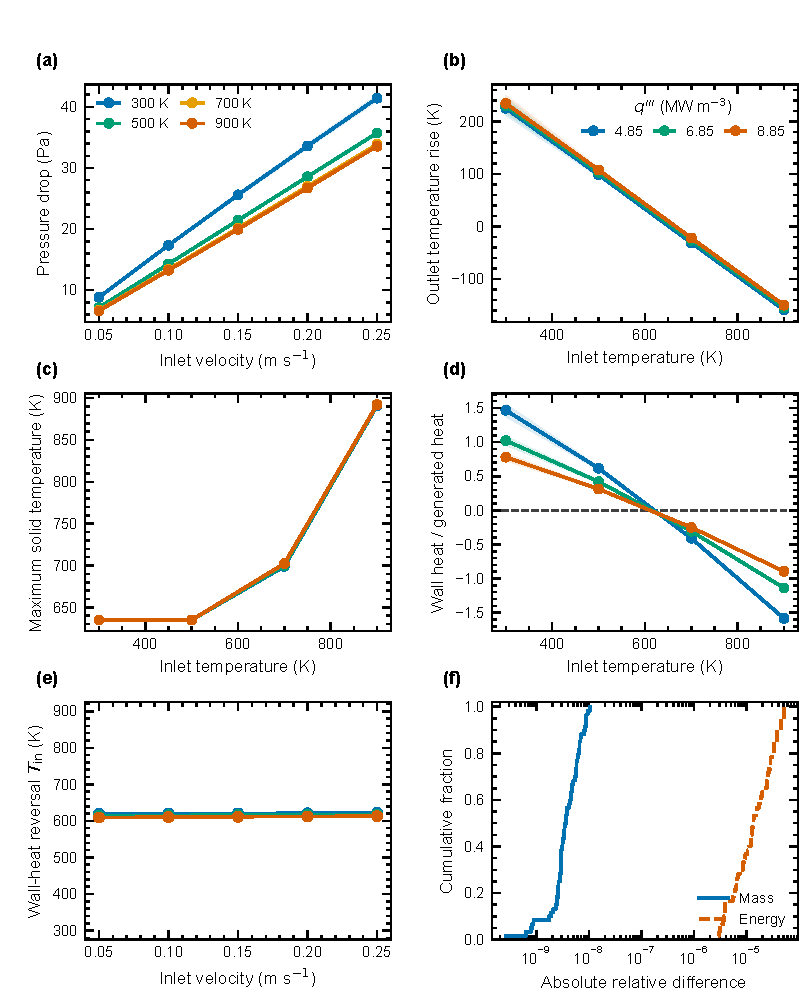
\includegraphics[width=\textwidth,height=0.75\textheight,keepaspectratio]{../figures/hccb_p418_physical_response.pdf}
\caption{Pore-resolved response across 60 conditions. (a) Pressure drop.
(b)--(d) Outlet-temperature rise, maximum solid temperature and normalized
signed wall heat; lines show medians and bands the sampled range.
(e) Inlet temperature at wall-heat reversal. (f) Mass and energy differences.}
\label{fig:physical_response}
\end{figure}
}{}

\IfFileExists{generated_steady_physics_text.tex}{%
\input{generated_steady_physics_text}}{}

\IfFileExists{generated_steady_final_windows.tex}{%
Across all 60 corrected-source-flow steady cases, the final 25 saved steady iterations changed the outlet temperature by at most \SI{0.0174}{K} and the maximum solid temperature by at most \SI{0.00212}{K}; among the 16 cases with paired full fields, the largest pointwise temperature change was \SI{0.0289}{K}.
}{}

\IfFileExists{generated_mesh_sensitivity.tex}{%
% Generated by code/build_hccb_p418_mesh_sensitivity_table.py
\begin{table*}[htbp]
\centering
\caption{Three-mesh sensitivity for the representative conjugate-heat-transfer condition. The equivalent cell size is $[(V_f+V_s)/(N_f+N_s)]^{1/3}$. Grid Convergence Index (GCI) values use the actual unequal refinement ratios and a safety factor of 1.25 \cite{celik2008gci}; no percentage GCI is reported for an oscillatory or unresolved sequence, or when the response crosses zero.}
\label{tab:mesh_sensitivity}
\small
\setlength{\tabcolsep}{4pt}
\resizebox{\textwidth}{!}{%
\begin{tabular}{@{}lrrrrrrr@{}}
\toprule
Grid & $N$ & $h_{\rm eq}$ ($\mu$m) & $\phi$ & $\Delta p$ (Pa) & $\Delta T_{\rm out}$ (K) & $\Delta T_{s,\max}$ (K) & $Q_{\rm wall}/Q_{\rm gen}$ \\
\midrule
Coarse & 361151 & 54.38 & 0.38591 & 23.3 & -26.52 & -0.1446 & -0.2733 \\
Medium & 947924 & 39.42 & 0.38661 & 25.64 & -26.2 & 0.05209 & -0.2942 \\
Fine & 1870064 & 31.43 & 0.38680 & 27 & -26.05 & 0.1608 & -0.3079 \\
\bottomrule
\end{tabular}
}
\par\vspace{0.5ex}
\resizebox{\textwidth}{!}{%
\begin{tabular}{@{}lrrr@{}}
\toprule
Quantity & Refinement behavior & Observed order & Fine-grid GCI \\
\midrule
Pressure drop & monotonic & 0.692 & 37.153\% \\
Outlet temperature rise & monotonic & 1.387 & 1.962\% \\
Maximum solid-temperature change & near-zero sign change & -- & -- \\
Signed wall heat / generated power & monotonic & 0.274 & 86.657\% \\
\bottomrule
\end{tabular}
}
\end{table*}


The three-grid comparison separates integral thermal convergence from local
hydraulic and wall-heat sensitivity. The fine-grid GCI is 1.96\% for outlet
temperature change, but 37.2\% for pressure drop and 86.7\% for signed
cooling-wall heat fraction. The maximum-solid-temperature change is close to
zero and changes sign across the three grids, so a percentage GCI is not
reported for that quantity. The common fine mesh therefore supports the
temperature-field model comparison, while pressure loss and wall heat are
retained as explicitly mesh-sensitive observables.}{}

\IfFileExists{generated_scope_limits.tex}{%
A separate full-domain fluid mesh failed the ordinary \texttt{checkMesh} test, so no solver was run on that mesh and no full-domain result is claimed. This limitation is distinct from the accepted local three-grid sensitivity study reported above. On the accepted local mesh, fixed-flow medium-to-fine thermal-curve differences remained below 0.043\%. Three fully coupled Courant-number tests stopped between \SI{0.000468}{s} and \SI{0.001105}{s} after pressure left the helium-property range; a run with consistent inlet velocity and mass flux similarly reached \SI{93413.3}{Pa}, below its \SI{93900}{Pa} limit. Model claims therefore concern thermal evolution with a prescribed hydrodynamic field. A direct OpenFOAM implementation of the same helium transport correlations was verified pointwise without a flow solve. A matched-initial representative using that implementation advanced to \SI{0.001522}{s} before a solid heat-capacity query reached \SI{1308.8}{K}, above the registered \SI{1300}{K} limit~\cite{kleykamp1996enthalpy}; this startup is used only to delimit property validity, not as fully coupled accuracy evidence.
}{%
The fixed-flow time-step study gave maximum medium-to-fine thermal-curve
differences below 0.043\%. Fully coupled startup calculations left the
specified helium-property pressure range before \SI{0.002}{s}; the model
results therefore concern thermal evolution with a prescribed hydrodynamic
field.}

\IfFileExists{generated_final_uncertainty_text.tex}{%
\input{generated_final_uncertainty_text}}{}

\subsection{External consistency checks}

\IfFileExists{../figures/hccb_heat_ai_external_evidence.pdf}{%
\begin{figure}[!htbp]
\centering
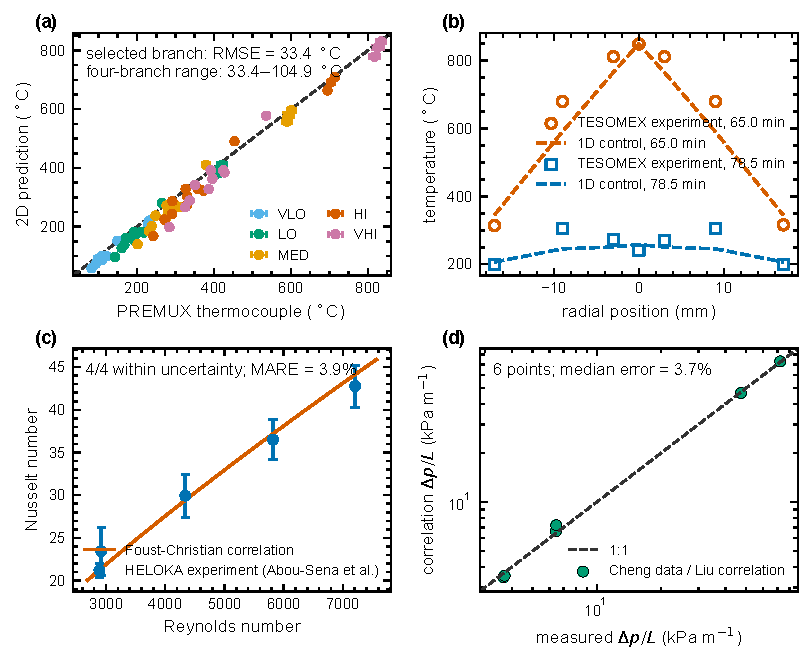
\includegraphics[width=\textwidth]{../figures/hccb_heat_ai_external_evidence.pdf}
\caption{External comparisons: (a) PREMUX thermocouples,
(b) TESOMEX radial temperatures, (c) HELOKA Nusselt numbers and (d) pressure
gradients in \SI{1}{mm} helium-cooled beds
\cite{hernandez2017premux,mohammed2018tesomex,abousena2023hcpb,
cheng2024pressure,liu2024unitary}. The data are not training labels.}
\label{fig:external_evidence}
\end{figure}
}{}

PREMUX and TESOMEX document spatial temperature structure that is not retained
by integral outlet measures. HELOKA and
fixed-bed data support the adopted convective and hydraulic scales, with mean
or median absolute relative errors of 3.9\% and 3.7\%, respectively. These
comparisons do not validate the specific three-dimensional packing.

\subsection{Sensitivity to pebble arrangement}

Nine matched conditions were recalculated on an independently generated
spherical-pebble arrangement. Relative to the source arrangement, the absolute
change is at most 0.67\% for outlet temperature and 0.31\% for maximum solid
temperature, but 14.7--18.0\% for pressure drop. Thus the integral thermal
response is comparatively robust for these two arrangements, whereas the
hydraulic response remains strongly geometry dependent
(Fig.~\ref{fig:cross_packing_integral}).

\IfFileExists{../figures/hccb_p418_seed202_integral_9.pdf}{%
\begin{figure}[htbp]
\centering
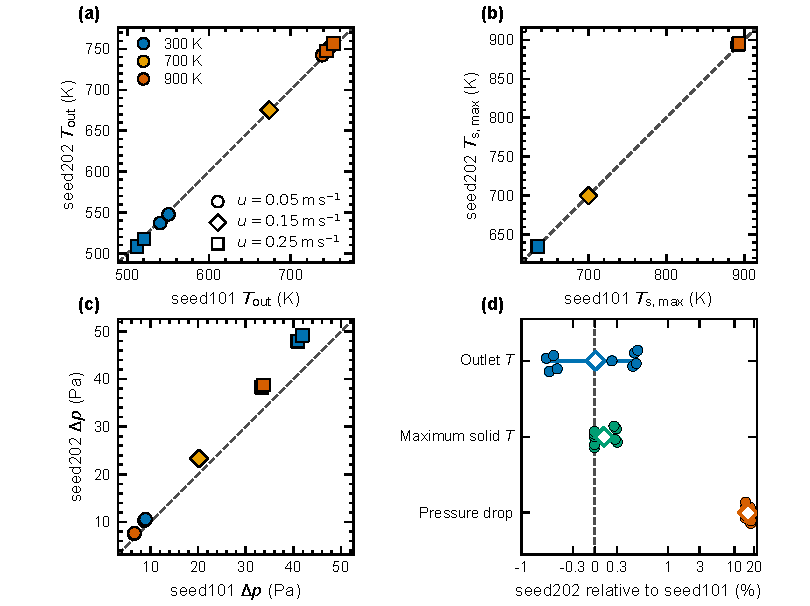
\includegraphics[width=\textwidth]{../figures/hccb_p418_seed202_integral_9.pdf}
\caption{Packing sensitivity at nine matched conditions. (a)--(c) Outlet
temperature, maximum solid temperature and pressure drop for seed101 and
seed202; the dashed line denotes parity, colors encode inlet temperature and
symbols encode inlet velocity. (d) Relative changes on a symmetric-logarithmic
axis (linear within $\pm1\%$); diamonds mark nine-condition means.
All points are direct calculations at the 200th steady nonlinear iteration.}
\label{fig:cross_packing_integral}
\end{figure}
}{}

\IfFileExists{generated_steady_model_comparison_validated.tex}{%
\subsection{Prediction of unseen steady conditions}
\IfFileExists{../figures/hccb_p418_steady_model_comparison.pdf}{%
\begin{figure}[!t]
\centering
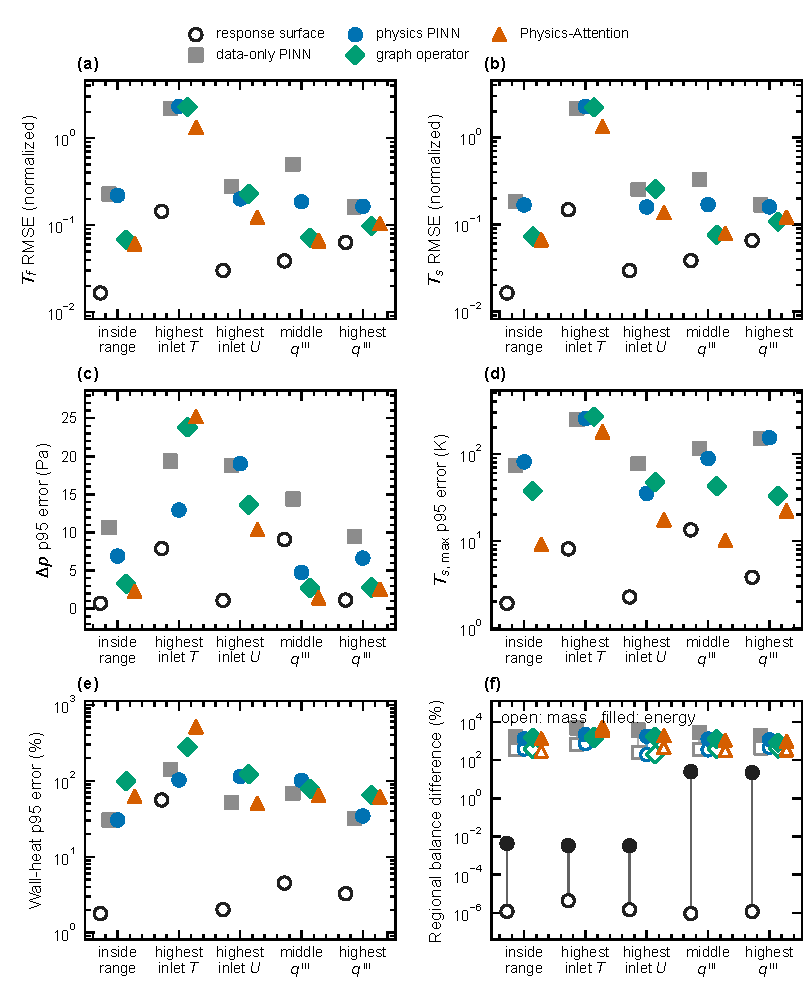
\includegraphics[width=\textwidth,height=0.75\textheight,keepaspectratio]{../figures/hccb_p418_steady_model_comparison.pdf}
\caption{Steady prediction on five complete-condition splits. Response-surface,
PINN, graph-operator and Physics-Attention models use identical temperature,
pressure, wall-heat and finite-volume balance measures.}
\label{fig:steady_model_comparison}
\end{figure}
}{}

\IfFileExists{generated_steady_performance.tex}{%
\begin{table*}[htbp]
\centering
\scriptsize
\setlength{\tabcolsep}{1.8pt}
\caption{Steady prediction accuracy and computational cost. Accuracy entries are the worst values across the five complete-condition splits in Figure~\ref{fig:steady_model_comparison}. Training and inference times are medians across the same five runs. The response-surface parameter range reflects validation-based selection between its linear and quadratic bases; neural-network parameter counts are fixed across splits. Times are measured values from the recorded computing device for each method and are not normalized to identical hardware.}
\label{tab:steady_performance}
\begin{tabular*}{\textwidth}{@{\extracolsep{\fill}}lrrrrrrr@{}}
\toprule
Method & \shortstack{Solid-$T$\\nRMSE} & \shortstack{Max-$T$ p95\\(K)} & \shortstack{Wall-heat p95\\(\%)} & \shortstack{Energy diff.\\(\%)} & \shortstack{Params\\(M; range)} & \shortstack{Train\\(min)} & \shortstack{Infer\\(ms)} \\
\midrule
response surface & 0.148 & 13.4 & 55.9 & 25 & 1.67--4.16 & 0.185 & 0.825 \\
data-only PINN & 2.17 & 246 & 140 & 4.89e+03 & 0.0368 & 0.878 & 4.93 \\
physics PINN & 2.27 & 253 & 114 & 2.2e+03 & 0.0368 & 0.898 & 5.14 \\
graph operator & 2.22 & 266 & 279 & 1.73e+03 & 1.45 & 20.7 & 116 \\
Physics-Attention & 1.33 & 178 & 510 & 5.41e+03 & 2.61 & 13.8 & 71.6 \\
\bottomrule
\end{tabular*}
\end{table*}
}{}
\IfFileExists{generated_steady_result_text.tex}{%
Across the five complete-condition splits, the lowest worst-case values for the six separately evaluated quantities are fluid-temperature nRMSE 0.144, solid-temperature nRMSE 0.148, pressure p95 error 9.07~Pa, solid maximum-$T$ p95 error 13.4~K, wall-heat p95 error 55.9~\%, regional energy difference 25~\%. All six are produced by the response surface; the separate quantities are not combined into a scalar model score.

With identical coordinate-network form, initialization, observations and optimization schedule, the data-only and physics-informed PINNs give, respectively, solid-temperature nRMSE 2.17 versus 2.27, wall-heat p95 error 140~\% versus 114~\%, regional energy difference 4.89e+03~\% versus 2.2e+03~\%. This paired comparison isolates the effect of the finite-volume mass, energy and interface-flux terms; all independent-condition values remain in Figure~\ref{fig:steady_model_comparison}.

The temperature-extrapolation split comprises training 30 conditions (30 wall-to-fluid, 0 fluid-to-wall), validation 15 conditions (0 wall-to-fluid, 15 fluid-to-wall), independent prediction 15 conditions (0 wall-to-fluid, 15 fluid-to-wall). It therefore measures transfer across the signed wall-heat change, not only interpolation between nearby inlet temperatures. The interleaved independent set contains 12 conditions (6 wall-to-fluid, 6 fluid-to-wall).

The two heat-source splits contain one training source level, so its zero-variance input is zero in every role; they test stability at unseen source levels, not learned source sensitivity.
}{}
\IfFileExists{generated_steady_seed_robustness_text.tex}{%
Across three independent initializations on the registered main split, the 
Transolver gives a solid-temperature nRMSE of $0.0675 \pm 0.0026$ and a maximum-solid-temperature p95 error of $11.9 \pm 1.2$~K.  The corresponding graph-operator values are $0.0725 \pm 0.0014$ and $27.1 \pm 8.9$~K.
This repeatability in temperature does not imply local energy closure: the Transolver wall-heat p95 error is $73.5 \pm 31.8$\%, and its mean regional energy-difference measure is $1321 \pm 63$\%.  The latter quantities are therefore retained as separate acceptance measures rather than being inferred from temperature accuracy.
}{}
}{}

\subsection{Prediction of held-out thermal trajectories}

Complete trajectories, rather than isolated time points, are withheld from
training and model selection. Persistence, DMDc, POD correction, diffusion
refinement and data-only or physics-constrained graph--Transformers are tested
on the same four endpoint pairs. Two temperature steps also withhold both
steady endpoints, testing the complete frozen steady-to-transient chain.

\IfFileExists{generated_transient_model_comparison_validated.tex}{}{%
\IfFileExists{generated_regional_dynamics_text.tex}{%
On the strict endpoint-pair holdout, repeating the initial temperature field gave fluid- and solid-temperature RMSE values of 3.63 and 3.55\,K, whereas continuous-time regional DMDc gave 5.45 and 5.03\,K. The lowest solid-field error was obtained by Initial-field persistence (3.55\,K), whereas the lowest hotspot p95 displacement was obtained by Initial-field persistence (2.48\,mm). These quantities are reported separately because a lower field-average temperature error does not by itself prove more accurate hotspot localization.
}{}
}

\IfFileExists{generated_transient_model_comparison_validated.tex}{%
\IfFileExists{../figures/hccb_p418_transient_model_comparison.pdf}{%
\begin{figure}[!htbp]
\centering
\includegraphics[width=\textwidth,height=0.75\textheight,keepaspectratio]{../figures/hccb_p418_transient_model_comparison.pdf}
\caption{Held-out thermal-trajectory prediction after validation-only model
and loss-weight selection. Solid-temperature responses to (a) velocity
increase, (b) velocity decrease, (c) heat-source increase and (d) heat-source
decrease. (e) Temperature error versus finite-volume energy-equation RMSE
after projection onto the common regional basis. (f) Accuracy versus
complete-chain speed-up relative to 32-rank \OpenFOAM{}; training and
data-generation costs are reported separately.}
\label{fig:transient_model_comparison}
\end{figure}
}{}
}{}

% The validated marker below supplies these values.  Empty fallbacks keep old
% preview metrics out of the manuscript source and are never typeset without
% that marker.
\providecommand{\PFieldModelLabel}{}
\providecommand{\PFieldFluidRMSE}{}
\providecommand{\PFieldSolidRMSE}{}
\providecommand{\PFieldFluidMaxError}{}
\providecommand{\PFieldSolidMaxError}{}
\IfFileExists{generated_openfoam_model_field_comparison_validated.tex}{%
\input{generated_openfoam_model_field_comparison_validated}
\IfFileExists{../figures/hccb_p418_openfoam_model_field_comparison.pdf}{%
\begin{figure}[!htbp]
\centering
\includegraphics[width=\textwidth,height=0.76\textheight,keepaspectratio]{../figures/hccb_p418_openfoam_model_field_comparison.pdf}
\caption{Regionalized OpenFOAM--model temperatures at \SI{25}{s} for an
independent test heat-source increase; the model was selected using validation trajectories only.
Rows: reference, \PFieldModelLabel{} prediction and
signed error; columns: fluid and solid phases. Reference and prediction
share a scale. Error colors are clipped at the 99th percentile; annotated
extrema and metrics are unclipped. Section interpolation is visual only;
metrics use the original regional nodes.}
\label{fig:field_cloud_comparison}
\end{figure}

The full regional-field fluid/solid RMSE in
Fig.~\ref{fig:field_cloud_comparison} is
\SI{\PFieldFluidRMSE}{K}/\SI{\PFieldSolidRMSE}{K}, and the corresponding
maximum absolute errors are \SI{\PFieldFluidMaxError}{K} and
\SI{\PFieldSolidMaxError}{K}.  These maxima are reported without color-scale
clipping, so the figure distinguishes representative spatial fidelity from
isolated extreme errors rather than reporting only an averaged score.
}{}
}{}

\IfFileExists{generated_transient_performance.tex}{%
\input{generated_transient_performance}}{}
\IfFileExists{generated_transient_result_text.tex}{%
\input{generated_transient_result_text}}{}
\IfFileExists{generated_fused_chain_text.tex}{%

\input{generated_fused_chain_text}}{}
\IfFileExists{generated_high_re_comparison.tex}{%
The three frozen graph--Transformer variants were additionally evaluated on
six independent high-velocity histories that were excluded from training,
normalization and model selection.  Their aggregate fluid/solid temperature
RMSE values are 122.6--\SI{123.9}{K} and
116.2--\SI{117.7}{K}, respectively; the fixed-weight physical residuals
do not improve this transfer.  Source steps remain within \SIrange{3.2}{6.3}{K}
and velocity steps within \SIrange{14.8}{21.0}{K}, whereas temperature steps
produce \SIrange{198.8}{215.9}{K}.  The dominant limitation is therefore
temperature-range extrapolation rather than flow-rate transfer alone.}{}
